\begin{frame}
  \frametitle{Linear Models}
  Objective: minimize error over all training data (squared, absolute, etc)
  \begin{equation}
    F(\boldsymbol{X}) = \beta_{0} +  \sum_{j=1}^{p} x_{j} \beta_{j}
  \end{equation}
  
  Regularization
  \begin{figure}[h!]
    \centering
    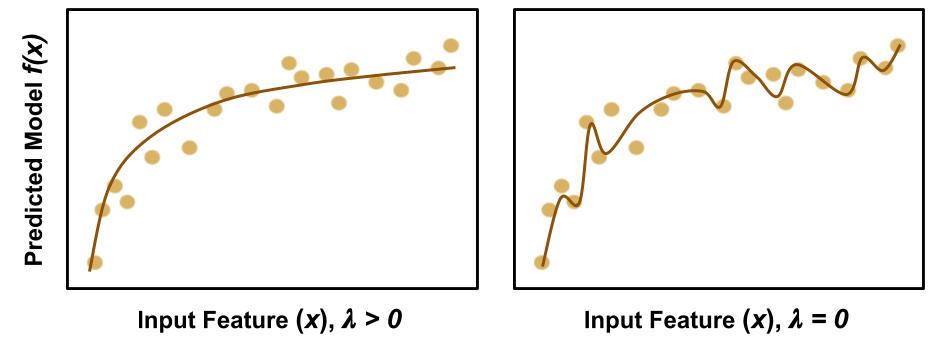
\includegraphics[width=0.9\textwidth]{./figures/regularization.png}
    \caption{Schematic of the impact of regularization on the generalizability of an ML model}
  \end{figure}
  \begin{equation}
    F(\boldsymbol{X}) = \beta_{0} +  \sum_{j=1}^{p} x_{j} \beta_{j} + \lambda \sum_{j=1}^{p} \beta_{j}^2
  \end{equation}
\end{frame}

\begin{frame}
  \frametitle{Nearest Neighbor Methods}
  Objective: minimum distance between test sample and training instance(s)
  \begin{equation}
    Y(\boldsymbol{X}) = \frac{1}{k} \sum_{x_i \in N_k(\boldsymbol{X})} y_i
  \end{equation}
  \begin{figure}[h!]
    \centering
    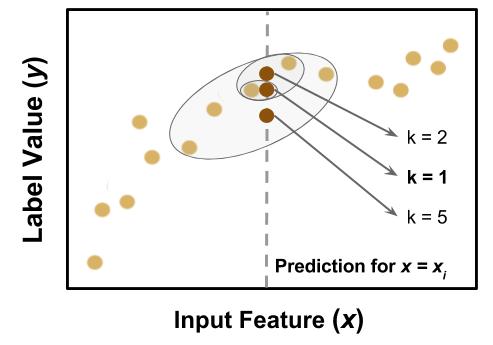
\includegraphics[height=0.5\textheight]{./figures/nn-fig.png}
    \caption{Illustration of the regularization effects by choosing \textit{k}}
  \end{figure}
\end{frame}

\begin{frame}
  \frametitle{Support Vector Machines}
  \begin{figure}
    \centering
    \begin{minipage}{0.5\textwidth}
      \centering
      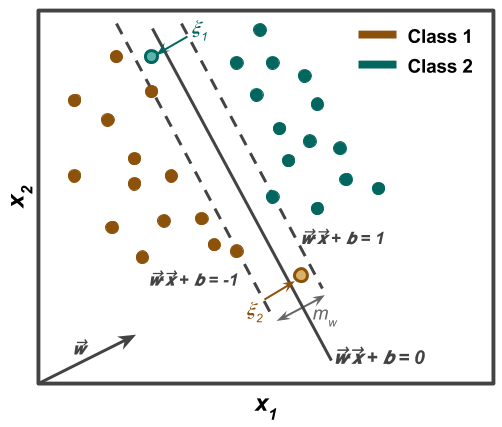
\includegraphics[width=\linewidth]{./figures/svm.png}
    \end{minipage}%
    \begin{minipage}{0.5\textwidth}
      \centering
      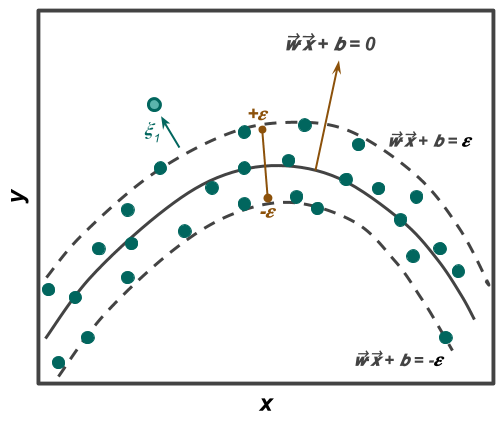
\includegraphics[width=\linewidth]{./figures/svr-a.png}
    \end{minipage}
    \caption{Classification with SVM and regression with SVR}
  \end{figure}
\end{frame}

\begin{frame}
  \frametitle{Support Vector Regression with Many Dimensions}
  \begin{minipage}{.5\textwidth}
    \centering
    \begin{figure}
      \centering
      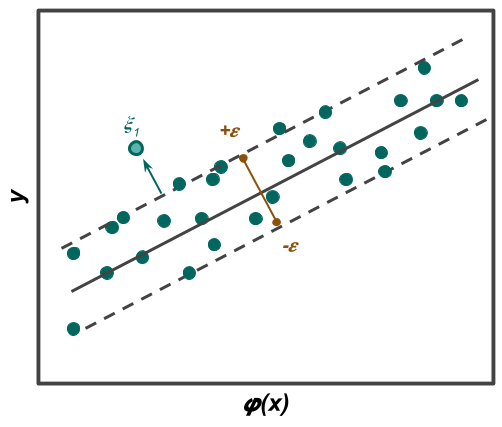
\includegraphics[width=\linewidth]{./figures/svr-b.png}
      \caption{Diagram showing the use of the kernel trick with SVR}
    \end{figure}
  \end{minipage}%
  \begin{minipage}{.4\textwidth}
    \centering
    \small
    \begin{equation}
      \begin{split}
        min\ & \frac{1}{2} \lVert w \rVert ^{2} + C \sum_{i} \xi_{i} \\
        subject\ to:\ \ & \lvert y_i - (w \phi(x_i) + b) \rvert \leq \varepsilon + \xi_i \\
        where:\ & w = \sum_{i} \alpha_i y_i \phi(x_i) \\
        and:\ & K(x_i, x_j) = \phi(x_i) \phi(x_j) = e^{\gamma \lVert x_i - x_j \rVert ^{2}}
      \end{split}
    \end{equation} 
    \normalsize
  \end{minipage}
\end{frame}

\begin{frame}
  \frametitle{Dimensionality Reduction}
  Manual via domain knowledge or some measure
  
  PCA

  Factor Analysis

  ICA
\end{frame}
